\section{Layout}
The layout module provides layout algorithms for laying out components. A component is an abstraction; it can be implemented in many ways, for example as items in a HTML5 Canvas drawing or as HTML elements. The module currently provides three layout algorithms: border, which lays out components in five different regions; grid, which lays out components in a user defined grid, and flex-grid which offers a grid with flexible column and row sizes.

The design of the layout module is inspired by the Java Swing layout managers \cite{sun08} and my own OpenGL based User Interface library \cite{stein06}. The module itself is not part of the core charting library but distributed as a separate library \cite{stein08} and bundled with a jQuery plugin for laying out HTML elements.

We start with the definition of a component; a component is something that has a minimum size, a preferred size, and a maximum size. It also has a method to set its size and position. A container is a component that contains other components and lays them out according to a layout algorithm (which are provided in the layout module.) Components need to satisfy the following interface requirements in order to be used with the layout algorithms; the component should have a:
\begin{itemize}
\item \code{bounds} property which returns the location and dimensions of the component;
\item \code{preferredSize}, \code{maximumSize}, and \code{minimumSize} properties which return the preferred, minimum and maximum size of the component respectively;
\item \code{insets} property which returns the offset between a container and its contents;
\item \code{isVisible} method which returns true if the component is visible;
\item \code{doLayout} method which might call a nested layout manager.
\end{itemize}

Note that the distinction between containers and components is artificial, both implement the same interface. 

\subsection{Border layout}
The border algorithm lays out components in five different regions. These regions are called center, north, south, east and west. The center component will be laid out in the center of the container, north on top of it, south beneath it and west and east on the left and right side respectively. The layout can only contain one of each region, but all are optional. Figure \ref{border} shows a visualization of a layout using all five regions. 

\begin{figure}[h!]
\centering
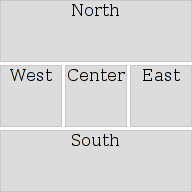
\includegraphics[width=.3\linewidth]{border}
\caption{Border layout with all five components present}
\label{border}
\end{figure}

The following example lays out a west, center and north component with a vertical space of 5 units between each component. There may be additional space between the components and the container if the container returns non-zero insets.
\begin{verbatim}
  var borderLayout = jLayout.border({
    west:   myWestComponent,
    center: myCenterComponent,
    north:  myNorthComponent,
    vgap: 5
  });

  borderLayout.layout(myContainer);
\end{verbatim}
If a region is not specified or the component is not visible its space will be taken up by the other components. 

\subsection{Grid layout}
The grid algorithms lays out the components in a grid, and resizes each component to the same size. The number of columns and rows can be specified by the user. Figure \ref{grid} shows a visualization of a grid layout with four components in a 2x2 grid. 

The following example lays out four components in a 2x2 grid, without any spacing between the components.
\begin{verbatim}
  var gridLayout = jLayout.grid({
    rows: 2,
    columns: 2,
    items: [myComponent1, myComponent2, myComponent3, myComponent4]
  });

  gridLayout.layout(myContainer);
\end{verbatim}

\begin{figure}[h]
\centering
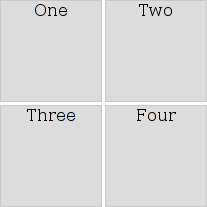
\includegraphics[width=.3\linewidth]{grid}
\caption{Grid layout with four components}
\label{grid}
\end{figure}

If the number of rows is given, the number of columns is calculated automatically by taking the number of components into account. If the number of rows is not given (or set to zero), and the number of columns is given, the number of rows will be automatically calculated using the number of components. If neither is given, the number of rows is set equal to the number of components and the number of rows is set to zero.

\subsection{Flex grid layout}
The flex grid algorithms lays out the components in a grid with flexible row and columns sizes. The number of columns and rows can be specified by the user. Figure \ref{flex-grid} shows a visualization of a flex grid layout with six components in a 3x2 grid. 

\begin{figure}[h]
\centering
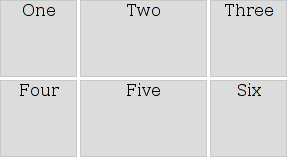
\includegraphics[width=.4\linewidth]{flexgrid}
\caption{Flex grid layout with six components}
\label{flex-grid}
\end{figure}

The interface to the flex grid is identical to that of the grid layout, and thus not further explained.
